\chapter{StencilFlow Implementation}



\section{Software Overview}
StencilFlow consists of many modules, some of them are very specific and dependent on others while we tried to keep many modules as general as possible for reuse within the tool. Figure \ref{fig:implementation-class-overview} gives you an overview how the different classes are nested and where they are instantiated.  
\begin{figure}[h]
	\centering
	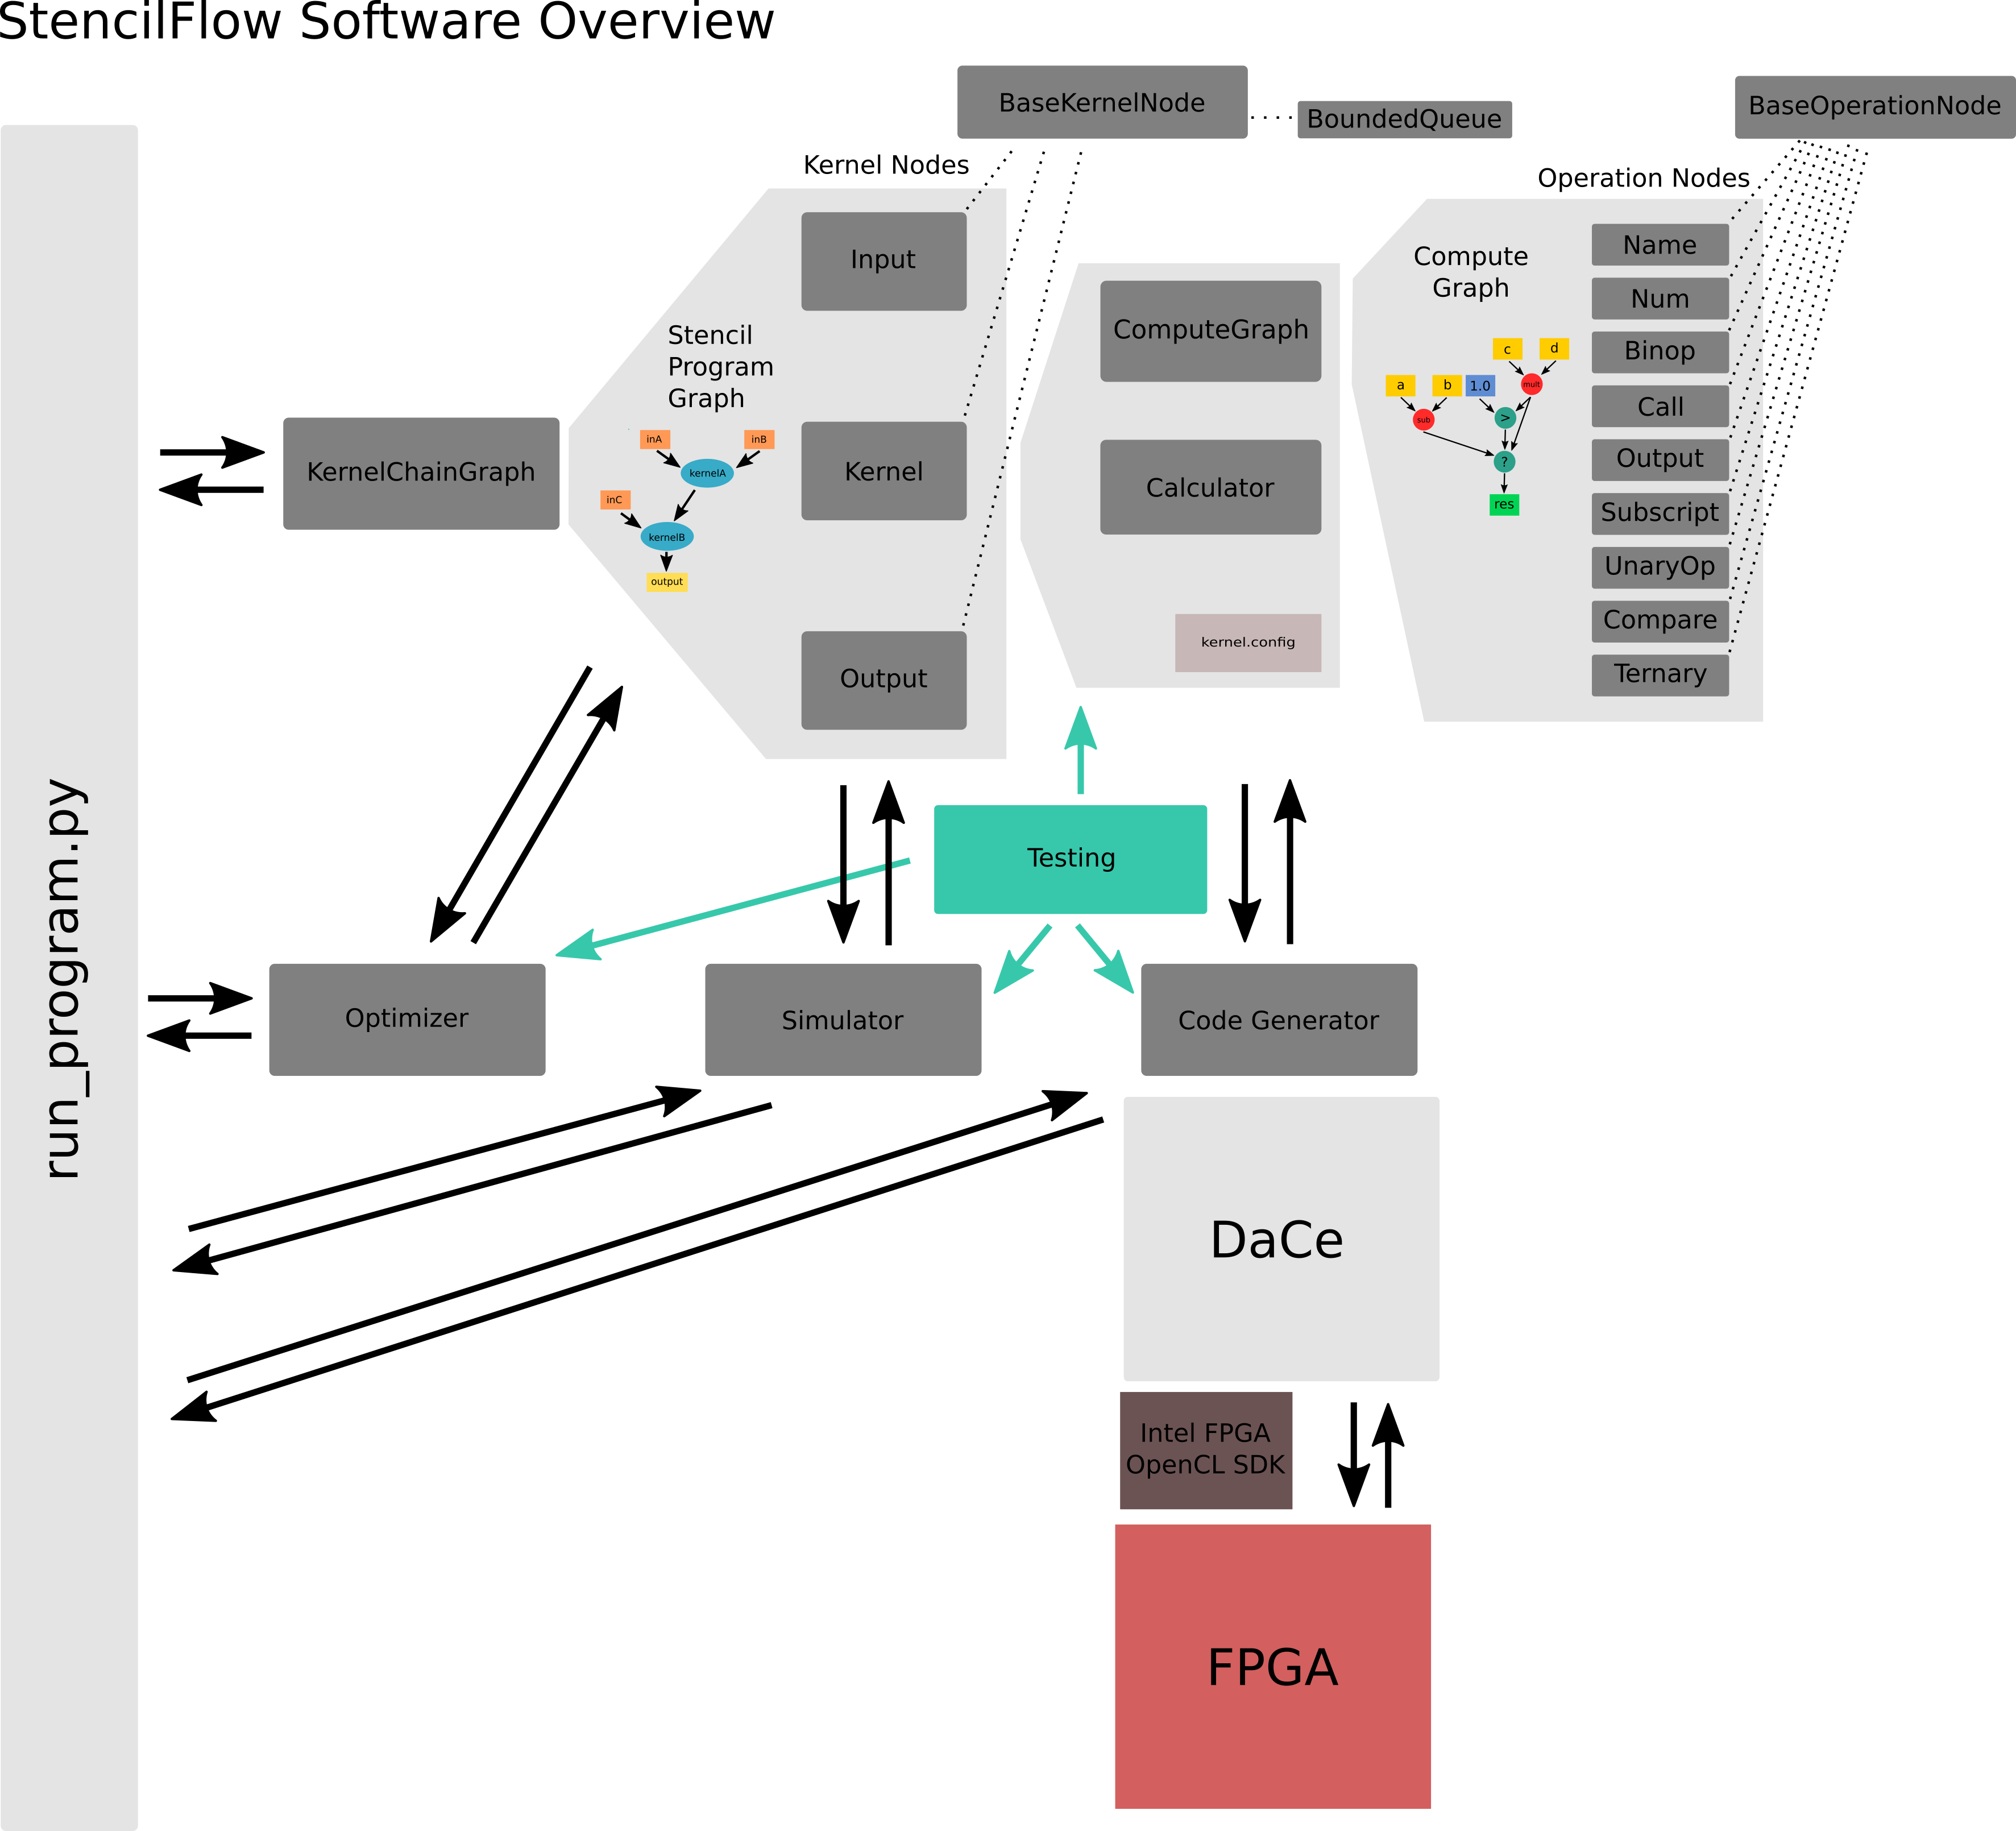
\includegraphics[height=24em]{drawings/implementation-class-overview.png}
	\caption{Overview of the StencilFlow class structure and their interaction.}
	\label{fig:implementation-class-overview}
\end{figure}
This section is dedicated to give you a detailed insight into the actual implementation with additional clarification why and how we implemented certain functionality.\\


This code snippet gives you an overview how the main classes interact with each other:
\begin{minted}{python}  
# instantiate the KernelChainGraph
chain = KernelChainGraph(path=args.stencil_file,
                         plot_graph=args.plot,
                         log_level=args.log_level)

# instantiate the Optimizer
opt = Optimizer(kernels=chain.kernel_nodes,
                dimensions=chain.dimensions,
                log_level=chain.log_level)
opt.optimize_to_ratio(1e-2)
    
# instantiate the Simulator
sim = Simulator(input_config_name=args.stencil_file
                chain=chain,
                write_output=False,
                log_level=args.log_level)
sim.simulate()
            
chain.report(args.stencil_file)
sim.report()
\end{minted}






\section{Input File}
The input json file contains all information required to analyze, optimize and run the given stencil program. We will go through its sections and explain them in detail.
\begin{minted}{json}
{
"inputs": {
    "inA": {
        "data": [
            19.30100000000000000e+00,
            19.43700000000000000e+00,
            19.30100000000000000e+00,
            19.03700000000000000e+00,
            19.36400000000000000e+00,
            19.31100000000000000e+00,
            19.93600000000000000e+00,
            20.10300000000000000e+00,
            20.24600000000000000e+00,
            20.03800000000000000e+00,
            20.36800000000000000e+00,
            20.03900000000000000e+00,
            20.24700000000000000e+00,
            20.03400000000000000e+00,
            20.10300000000000000e+00,
            20.56400000000000000e+00,
            20.94800000000000000e+00,
            19.19300000000000000e+00,
            19.36700000000000000e+00,
            19.98700000000000000e+00,
            20.43200000000000000e+00,
            20.95200000000000000e+00,
            21.34400000000000000e+00,
            21.07300000000000000e+00
        ],
        "data_type": "float64"
    },
    "inB": {
        "data": "inB.csv",
        "data_type": "float64"
    },
    "inC": {
        "data": "inC.dat",
        "data_type": "float32"
    }
},
"outputs": [
    "kernelB"
],
"dimensions": [
    2,
    3,
    4
],
"program": {
    "kernelA": {
        "computation_string": "out = 3.14 * (inB[i,j,k]-inB[i,j-1,k]);
                               res = (inA[i,j,k] + out) * cos(out);",
        "boundary_condition": {
            "inA": {
               "type": "constant",
               "value": 1.0
            },
            "inB": {
                "type": "constant",
                "value": 7.5
            }
        },
        "data_type": "float64"
    },
    "kernelB": {
        "computation_string": "res = kernelA[i,j,k] + inC[i,j,k];",
        "boundary_condition": {
            "kernelA": {
                "type": "copy"
            },
            "inC": {
                "type": "copy"
            }
        },
        "data_type": "float64"
    }
}
}
\end{minted}

\paragraph{Inputs}
The inputs section is dedicated to the input data arrays. For each input data array, there exists an entry that either contains data directly or references to an external file in binary or csv format. Furthermore, it specifies the data type and precision of the data.


\paragraph{Outputs}
The output section contains all kernel names of which data should not be discarted, but rather written back to the host computer as the output or computation result. This list can contain a single item or multiple entries.


\paragraph{Dimensions}
The dimensions value represents the global problem size and should correspond to the dimensions of the data arrays too (e.g. dimX*dimY*dimZ = size(input array)).


\paragraph{Program}
The program section contains information about the kernels of the stencil program. The computation\_string represents the kernel computation. The boundary condition subsection defines the condition per input in case of an out-of-bound data read. The data type specifies the precision of the computation. \\
\textit{Note: The precision value of data\_type might have severe performance impact  due to the impact in buffer requirements and the usage of hardened floating point operators.}






\section{Bounded Queue (bounded\_queue.py)}
The BoundedQueue class represents the basic building block when it comes to handle data in a FIFO manner. It can act as a feed to push data into the pipeline (input nodes), connect stencil chains as channels (internal and delay buffer), it does latency simulation within the kernel and collects all final results to store them on disk. We will go through the implementation details and explain for what the functionalities are useful. 

\begin{figure}[h]
	\centering
	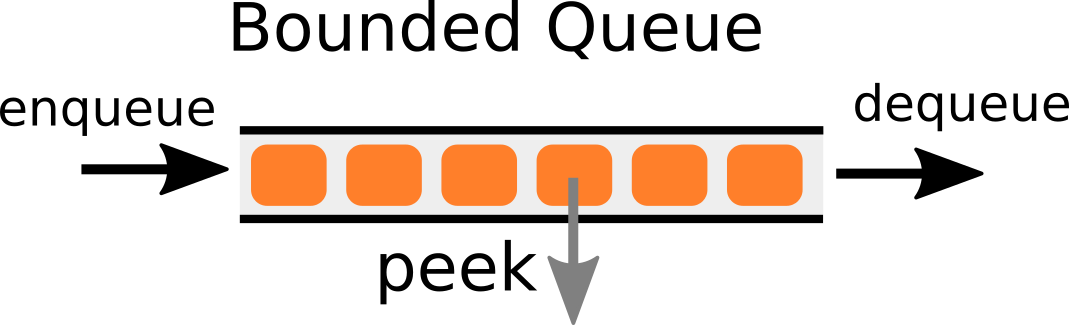
\includegraphics[height=8em]{drawings/implementation-bounded-queue.png}
	\caption{Working principle of the bounded queue implementation.}
	\label{fig:implementation-bounded-queue}
\end{figure}

\paragraph{Generic}
There are several short-cut implementations for generic functionality necessary to work with these data structures such as getting the actual size, check if the data structure is full respectively empty or print the basic instance info in a well-arranged way.


\paragraph{dequeue / try\_dequeue}
Removing and retrieving a single element from the BoundedQueue can be achieved using the dequeue method. The difference between the two implementations lies in the error handling. In case of an empty queue, dequeue raises an exception while the try\_dequeue method simply returns False instead of a data element in case of an empty queue. \\

There are valid use cases for both of them. For example in case of a kernel program trying to read data from input channels, that might or might not be available yet, try\_dequeue might be the better choice to avoid having to handle the exception.


\paragraph{enqueue / try\_enqueue}
Adding a single element to the BoundedQueue can be achieved using the enqueue method. The difference between the two implementations lies in the error handling. In case of a full queue, enqueue raises an exception while the try\_enqueue method simply discards the data item and indicates success or failure by the boolean return value. 


\paragraph{peek / try\_peek\_last}
The peeking functionality allows to retrieve items add arbitrary positions in the queue without actually removing them from the queue. Especially try\_peek\_last is very useful for the simulator to read the next element that is being feed into the kernel without actually touching the data.


\paragraph{import\_data / export\_data}
For the initial setup and cleanup we usually have to add many elements to a queue or retrieve all data elements from it. These functionalities are provided by the import\_data respectively export\_data methods.





\section{Calculator (calculator.py)}
The Calculator class provides the service of given a mathematical expression and a map from all variables to their corresponding values, to compute the numerical result of the expression, even for conditional expressions in the form of \textit{if(condition) true\_expression else false\_expression}. 

\paragraph{Internals}
The functionality is implemented by first parsing the expression into an abstract syntax tree. This tree is used later on to walk through and compute the intermediate values leading to the final result by having custom AST tree walker functions implemented. 
\begin{figure}[h]
	\centering
	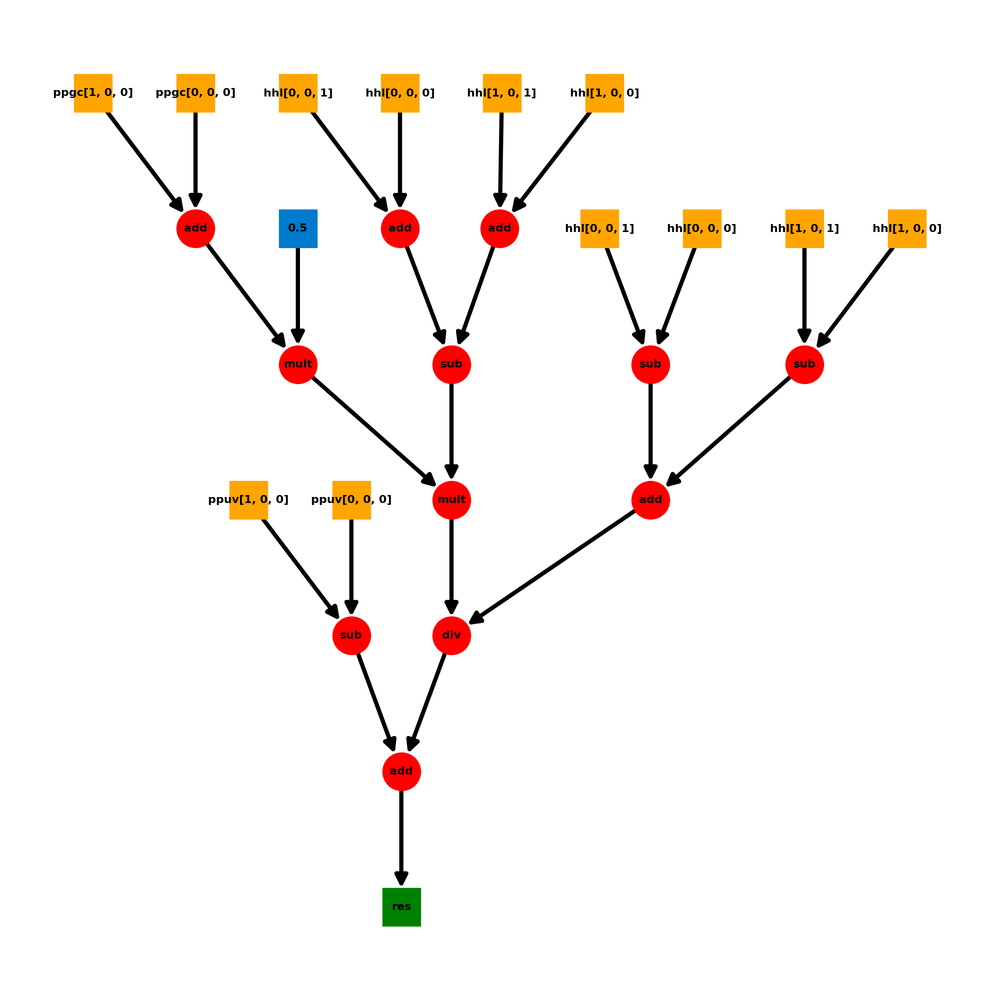
\includegraphics[height=16em]{images/compute-graph-example.png}
	\caption{Example of the high level visualization of a abstract syntax tree compute graph.}
	\label{fig:compute-graph-example}
\end{figure}


\paragraph{eval\_expr}
The Calculator class provides a single method for evaluation of an expressing. Given a mathematical expression and a map of all variable names to its corresponding value, the calculator computes the final result. This functionality is required for the simulator to be able to compute the kernel result, given all input values.


\paragraph{Example Usage}
The following example should illustrate the functionality of the Calculator class.
\begin{minted}{python}
variables = dict()                                
variables["a"] = 7                                
variables["b"] = 2                                

for var in variables:                             
  print("name: {}, value: {}"
        .format(var, str(variables[var])))

computation = "cos(-a + b) if (a > b) else (a + 5)
calculator = Calculator()                         
result = calculator.eval_expr(variables, computati
print("{} = {}".format(computation, str(result))) 
\end{minted}
Returns:
\begin{lstlisting}[showstringspaces=false, frame=single, language=Python]
name: a, value: 7
name: b, value: 2
cos(-a + b) if (a > b) else (a + 5) * b = 0.28366
\end{lstlisting}






\section{Compute Graph Nodes (compute\_graph\_nodes.py)}
The ComputeGraphNodes implement the BaseOperationNodeClass and are nodes of the ComputeGraph. Their main functionality beside have different nodes types in the three is to generate names and symbols for visualization from the given abstract syntax tree node. \\

\textit{Name}: The Name node class represents the variable name node in the computation tree. \\

\textit{Num}: The Num node class represents the numeral node (constant values) in the computation tree.\\


\textit{Binop}: The Binop node class represents the binary operations (e.g. addition, subtraction, etc.) in the computation tree.

\textit{Call}: The Call class represents the function calls (e.g. sin/cos,..) nodes in the computation tree. We support functions with single arguments, which could be extended to multiple argument functions if necessary.\\

\textit{Output}: The Output class represents the output node in the computation tree. \\

\textit{Subscript}: The Subscript class represents the array field access nodes in the computation tree. (e.g. inX[i,j,k+1]). It does convert the [i,j-2,k+1] index to relative number indices i.e. [0,-2,1] \\

\textit{Ternary}: The Ternary operator class represents ternary operation of the form:
expression\_true if comparison\_expression else expression\_false \\

\textit{Compare}: The Comparison operator class represents the comparison of two expression by a comparator (e.g $=, >=$, ..).

\textit{UnaryOp}: The UnaryOp operator class represents unary operations. In our case we only support negation (mathematical - sign) as unary operation yet.





\section{Compute Graph (compute\_graph.py)}
The ComputeGraph class represents the actual computation of a kernel instance. It analyses the field access patterns and metrics such as the critical path latency. Furthermore, it generates a high-level graph representation from the input fields through the computational nodes to the output, which can be visualized nicely.


\paragraph{Configuration}
Performance metrics such as latency greatly depends on the underlying FPGA hardware. This is why we did not hard-code such values, but rather provide the flexibility to load the configuration of operation latency values at runtime. 
\begin{minted}{json}
{
"op_latency": {
	"add": 16,
	"sub": 16,
	"mult": 16,
	"div": 128,
	"inv": 16,
	"sin": 128,
	"cos": 128,
	"tan": 128,
	"sinh": 128,
	"coshh": 128,
	"comparison": 16,
	"conditional": 16,
	"neg": 16
	}
}
\end{minted}


\paragraph{Nodes}
The computation graph contains several different node types, each of them represents either a data source, a data destination or some type of computation.
\begin{itemize}
	\item Name: variable names
	\item Num: numeral (constant number)
	\item Binop: binary operation (e.g. addition, subtraction etc.)
	\item Call: function call (e.g. sin(), cos(), etc.)
	\item Output: output/result node
	\item Subscript: array access (e.g. inX[i,j,k+1])
	\item Ternary: ternary (conditional) operation node of the form: if\_expr if condition else else\_expr
	\item Compare: part of the ternary operator, tests the condition
	\item UnaryOp: unary operations (e.g. negation)
\end{itemize}


\paragraph{setup\_internal\_buffers}
This method takes care of computing the internal buffer size. This can be achieved by first finding the highest and the lowest access index per field and compute the difference which is exactly the internal buffer size plus one. internal buffer size(field) = max\_field\_access(field) - min\_field\_access(field) + 1.


\paragraph{Data Reuse, Multiple Expressions}
There are many cases where part of the kernel expression is occurring more than one time. For efficiency reasons, it makes sense to compute them only once. We provide this functionality by allowing to split the expression into subexpression, which can be referenced multiple times. This can be achieved using the following syntax: "res = -a if (a+1 $>$ b-c) else b; b = d + e" where b is being substituted twice by (d + e). \\
From the implementation perspective, we have to account for the processing of both parts of the expression as well as contracting the output node b (from b = d + e) with the input node b (in res = -a if (a+1 $>$ b-c) else b;), which is being achieved by the contract\_edge method.


\paragraph{generate\_graph}
The generate\_graph method creates a high-level networkx graph consisting of OperationNodes for further visualization and analysis. The expression is parsed using the abstract syntax tree framework which gives us the ability to walk through the AST tree in order to extract all the required information.
The ast\_tree\_walk method is a recursive method that does the following steps:
\begin{enumerate}
	\item create a new node from node and the node number and add it to the graph
	\item depending on the type of node, call ast\_tree\_walk recursively for left child (node number: 2*parent + 1) and right child (node number: 2*parent)
	\item add edge from the new node to the recursive 
	child/children
	\item return new node
\end{enumerate}
% ref to networkx


\paragraph{plot\_graph}
Visualizing the problem instances greatly helps to get a good understanding of the problem and seeing what is going or what we could further optimize. This method accounts for that by plotting a well-arranged overview of the ComputeGraph. 
\begin{figure}[h]
	\centering
	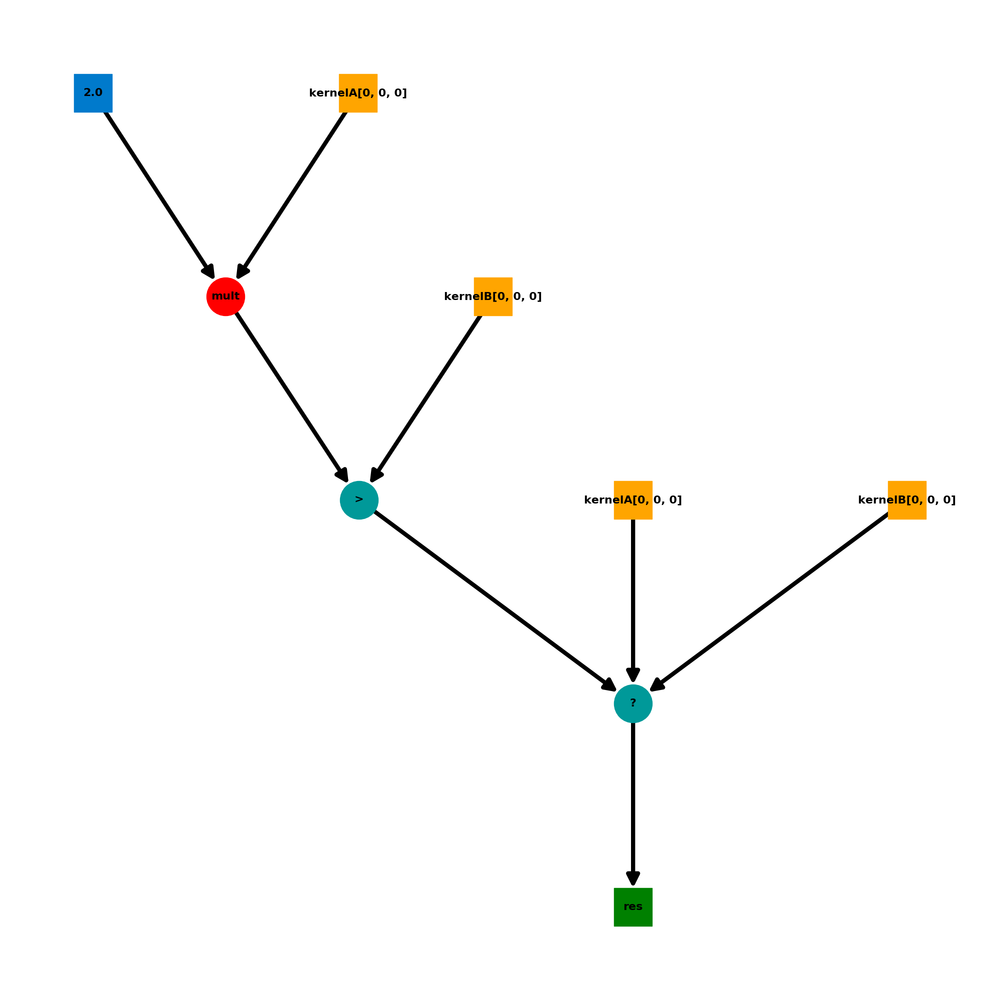
\includegraphics[height=16em]{images/compute-graph-debugging-example.png}
	\caption{Example of the high level visualization of a abstract syntax tree compute graph.}
	\label{fig:compute-graph-debugging-example}
\end{figure}


\paragraph{calculate\_latency}
The latency of the critical path is a key metric for our problem question and part of the ComputeGraphs functionality. This can be achieved by a recursive tree walk from the output node up to the field accesses while carrying out the latency propagation i.e. latency\_to\_outp(child) = max\{latency\_to\_outp(child), latency\_to\_outp(self) + operation\_latency(self)\}
\textit{Remark: The reason for using the maximum of both values is that the tree is not a classical mathematical tree, but rather a directed acyclic graph. It can happen due to the allowance of substitution/reuse of identical part of the computation to have a cycle if we look at it as an undirected graph. This behavior can be seen by the example ComputeGraph above.}







\section{Base Node (base\_node\_class.py)}
The base node class is not a class by itself, but rather contains the abstract base nodes for the ComputeGraph and the KernelChainGraph. \\


\paragraph{BaseKernelNodeClass}
The BaseKernelClass provides all the basic fields and functionality for its subclasses which are the Input, Kernel and Output classes. These are nodes of of the KernelChainGraph. \\
Furthermore, it provides a fall-back implementation of the generate\_label functionality.


\paragraph{BaseOperationNodeClass}
The BaseOperationNodeClass class provides all the basic fields and methods for its subclasses (Num, Subscript,..). These are the nodes of the ComputeGraph.\\
Furthermore, it provides a fall-back implementation of the generate\_label and functionality. In addition, it contains an method generate\_name to generate the node name from the AST node, which all subclasses have to implement.








\section{Input (input.py)}
The Input class is a subclass of the BaseKernelNodeClass and represents an Input node in the KernelChainGraph. Its purpose is to feed input data into the pipeline/data flow design. 


\paragraph{init\_queues}
This method sets up a dedicated queue for each output channel. This is necessary since some of the kernels might have to wait for other inputs to get available till they start reading from this channel.


\paragraph{try\_write}
This method is called by the simulator in the step execution cycle. The input node loops over all output channels and tries to add a data element to them. If the corresponding data queue is already empty (all elements already feed) it inserts a "bubble" (None) in order to keep the data flow running. If the output channel is full, it does nothing. 
\begin{figure}[h]
	\centering
	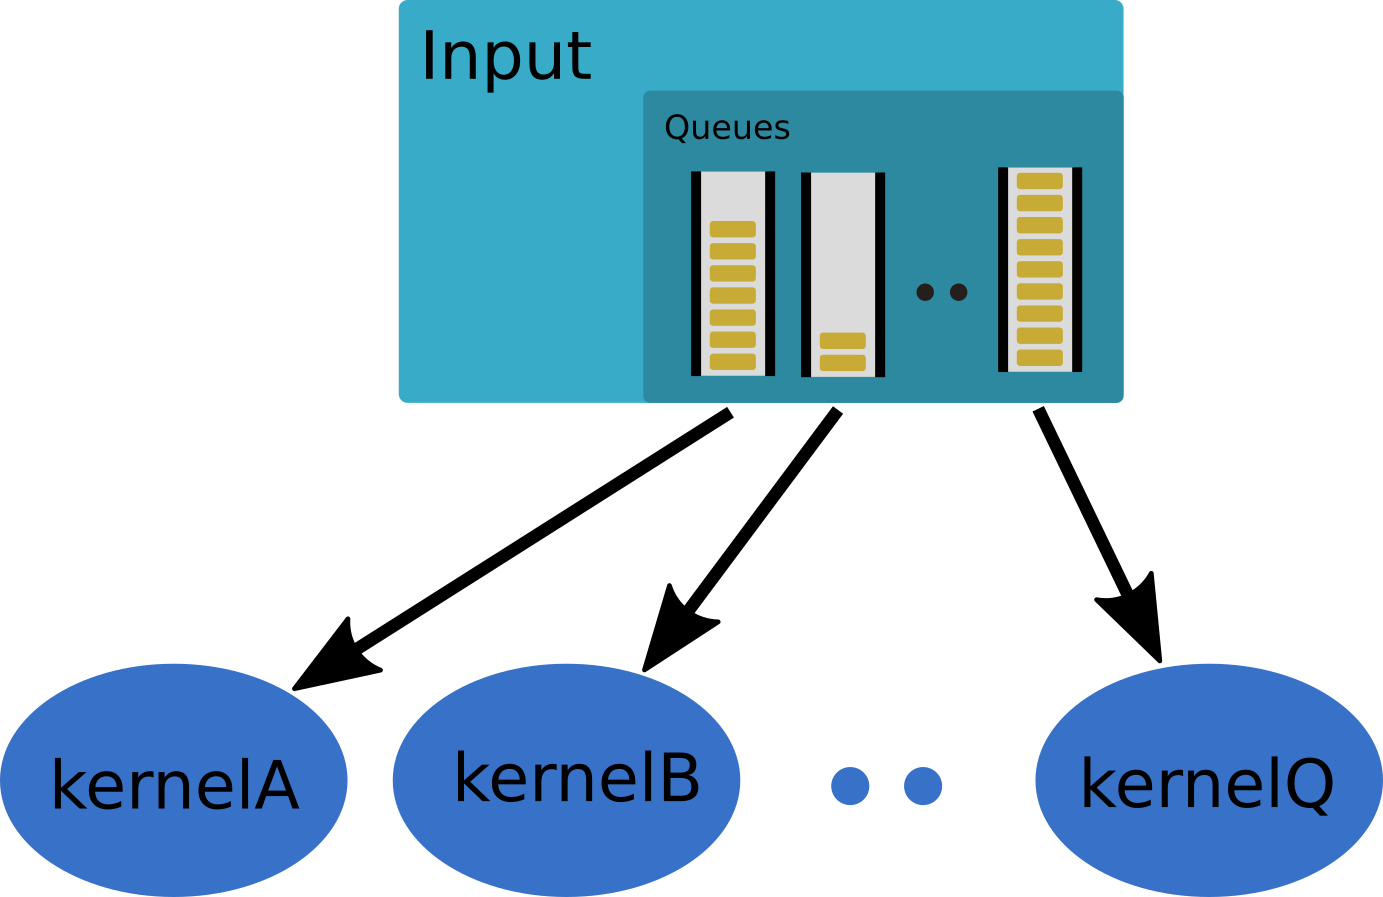
\includegraphics[height=16em]{drawings/inputs-multi-queue.png}
	\caption{The functionality of the Input node. Feed each channel individually.}
	\label{fig:inputs-multi-queue}
\end{figure}


\paragraph{init\_input\_data}
The init\_input\_data method initializes the internal queues with data from the config file or the file system. It currently supports the following file types: implicit (array defined in the input config file), binary (.dat, .bin, .data) , h5 and csv.







\section{Output (output.py)}
The Output class is a subclass of the BaseKernelNodeClass and represents an Output node in the KernelChainGraph. Its purpose is to store data coming from the pipeline/dataflow design. 


\paragraph{try\_read}
This method is called by the simulator in the step execution cycle. It simply tries to read from the input channel and stores the element into the data\_queue on success.


\paragraph{write\_result\_to\_file}
The write\_result\_to\_file method writes the content of the internal queue with the computation results to the binary file at \textit{results/INPUT\_CONFIG\_NAME/SELF.NAME\_simulation.dat}. This can be used for example to compare the simulator values with the result coming from the actual hardware implementation.







\section{Kernel (kernel.py)}

\paragraph{Overview}
The Kernel class is used for four different scenarios:
\begin{enumerate}
	\item Initialization: setup and computation of buffer sizes and latencies.
	\item Optimization: set/reset swap out buffer flags
	\item Simulation: run data through the data flow graph by repeatedly calling try\_read/try\_execute and try\_write
	\item Code Generation: extraction of equations and buffer swap out flag
\end{enumerate}


\subparagraph{Initialization}
The initialization phase looks like:
\begin{enumerate}
	\item instantiate Calculator class
	\item instantiate ComputeGraph class with given compute\_string
	\item generate compute graph (networkx data structure)
	\item compute compute graph latency (critical path)
	\item compute and set up internal buffers
	\item set up latency simulation out delay queue
	\item compute access distance from furthest access to the center
\end{enumerate}


\subparagraph{Optimization}
The optimization framework takes kernels as input and sets or resets the field \textit{swap\_out} of the delay buffer or internal buffer parts to indicate whether or not the buffer should stay in fast memory.


\subparagraph{Simulation}
The simulator makes us of the pre-defined step execution calls \textit{try\_read, try\_execute} and \textit{try\_write}. 


\subparagraph{Code Generation}
The code generator makes use of the function \\*
\text{generate\_relative\_access\_kernel\_string} that transforms the input compute\_string with given global dimensions to a single dimensional index based string.
\begin{lstlisting}[showstringspaces=false, frame=single, language=Python]
dimensions are: [100, 100, 100]
input: res = a[i+1,j+1,k+1] + a[i+1,j,k] + 
             a[i-1,j-1,k-1] + a[i+1,j+1,k] + 
             (-a[i,j,k])
relative_access_kernel_string: res = ((((a[0] +
             a[-101]) + a[-20202]) + a[-1]) + 
             (-a[-10101]))
\end{lstlisting}



\paragraph{print\_kernel\_performance}
This methods pretty-prints the performance metrics (maximum buffer usage, average buffer usage, total execution time, etc) gathered during the simulation. 


\paragraph{update\_performance\_metric}
This method is called by the simulator every step execution in order to gather and process internal state metrics.


\paragraph{set\_up\_dist\_to\_center}
Computes for all fields/channels the distance from the furthest field access to the center of the stencil ([0,0,0]). \\ 
This is necessary and covers the following edge case: Suppose we have the kernel: \textit{out[i,j,k] = in[i,j,k-2] + in[i,j,k+2]} without accessing the center element (in[i,j,k]) from the input. We look at the time two step execution cycles before the first actual execution of this kernel with valid input data. The front access is already in the position to read valid data while the back access is in the boundary condition which can lead to an invalid execution (if no center access is used it seems to be valid but in fact is not). In order to circumvent this, we introduce the distance-to-center and decrement it every step to make sure we start as soon as the center element is in the first position.  
\begin{figure}[h]
	\centering
	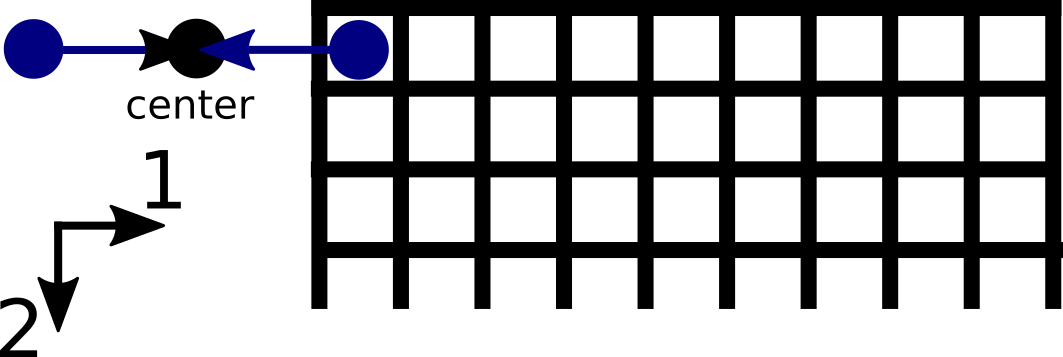
\includegraphics[height=8em]{drawings/software-dist-to-center.png}
	\caption{Edge Case: Distance to center.}
	\label{fig:software-dist-to-center}
\end{figure}


\paragraph{iter\_comp\_tree}
This method iterates through the computation tree in order to generate the kernel string (according to some properties e.g. relative to center or replace negative index. The pseudo code for the function is:
\begin{algorithm}
	\caption{iter\_comp\_tree(node)}
	\begin{algorithmic}
		\STATE get all predecessors pred
		\STATE check what type of Node node is
		\STATE depending on the node type, recursively call iter\_comp\_tree for the predecessor(s)
		\STATE return the formated string e.g. for binary operation: LHS op RHS
	\end{algorithmic}
\end{algorithm}
\textit{Relative to center: The absolute array index value is either relative to the center node e.g. center is at 0 and [i,j,k+10] is at [10] or relative to the front access e.g. the center is at [-10] and [i,j,k+10] is at [0].}
\\
Replace negative index: In order to get a valid variable name string, we have to replace the negative sign '-' by 'n' otherwise it gets interpreted as a mathematical symbol (for the Calculator class) e.g. arrA\_-20 gets replaced by arrA\_n20


\paragraph{generate\_relative\_access\_kernel\_string}
Generates the relative (either to the center or to the furthest field access) access kernel string which is necessary for the code generator HLS tool.


\paragraph{reset\_old\_compute\_state}
This is a helper function for the simulator to make sure that no artifacts from any previous simulation step is remaining. It clears the variable to value map and all execution related flags such as read\_success.


\paragraph{convert\_3d\_to\_1d}
Converts [i,j,k] to a flat 1D array index using the given dimensions [dimZ, dimY, dimX] using the formula:
index = i*dimY*dimX + j*dimX + k = (i*dimY + j)*dimX + k (dimensional to absolute value formula from the model part).


\paragraph{remove\_duplicate\_accesses}
The list of field accesses must be cleaned from duplicate entries, since they can be handled concurrently and could increase the complexity of the computations of StencilFlow.


\paragraph{setup\_internal\_buffers}
This method creates and splits the internal buffers according to the pipeline model. Each internal buffer part has the length from one access of the field to the next. This is done in the following way:
\begin{algorithm}
	\caption{setup\_internal\_buffers}
	\begin{algorithmic}
		\STATE sort all buffer accesses in the list
		\STATE case single buffer access: internal buffer is size 1
		\STATE case multiple buffer accesses: iterate over the list
		\STATE compute difference from current to next access
		\STATE create buffer of this size and add it to the buffers
	\end{algorithmic}
\end{algorithm}


\paragraph{buffer\_number}
Computes the index position of the internal buffer part from the access position. \\
\textit{Example: out[i,j,k] = in[i,j,k-10] + in[i,j,k] + in[i,j,k+10] has two internal buffers (form k-10 to k, and from k to k+10). The data item for the access [i,j,k+10] comes from the delay buffer, the one for [i,j,k] form the first internal buffer and for [i,j,k-10] from the second internal buffer. If we call buffer\_position([i,j,k+10]) we get '-1' which indicates the delay buffer. For buffer\_position([i,j,k]) we get '0' and for buffer\_position([i,j,k-10]) we get '1'}


\paragraph{get\_global\_kernel\_index}
Return the current position (simulator, program counter) within the computation as a list of the form [i,j,k]. This is required for the simulation to test if the data at a specific index is out-of-bound or not.\\
\textit{Example: global problem size: [2,3,4]. \\
	(1) Current program counter index: 3, global kernel index: [0,0,3] \\
	(2) Current program counter index: 7, global kernel index: [0,1,3]}


\paragraph{is\_out\_of\_bound}
Checks whether the current access is within bounds or not. This is required for the simulation to check if boundary conditions must be applied or regular data should be read.


\paragraph{get\_data}
Returns data of current stencil access (could be real data or boundary condition)


\paragraph{test\_availability}
This method checks if all accesses are available (and ready for execution). In addition, the method returns all accesses that are not available yet. Checks are different for different data types:

\subparagraph{Numeral (Constant Values)}
They are always available and therefore nothing has to be checked.

\subparagraph{Subscript (array) data accesses}
The buffers have to be checked if data is ready yet:
\begin{algorithm}
	\caption{setup\_internal\_buffers}
	\begin{algorithmic}
		\STATE peek the last element of the delay buffer
		\STATE peek the last element of all internal buffer junks
		\IF {none of the is 'None'}
		\STATE all data elements are available
		\ELSE
		\STATE not all items are available yet
		\ENDIF
	\end{algorithmic}
\end{algorithm}


\paragraph{move\_forward}
Moves all items within the internal and delay buffer one element forward to free up space for a new data element. The furthest element is getting discarded since it is not used anymore.  
\begin{figure}[h]
	\centering
	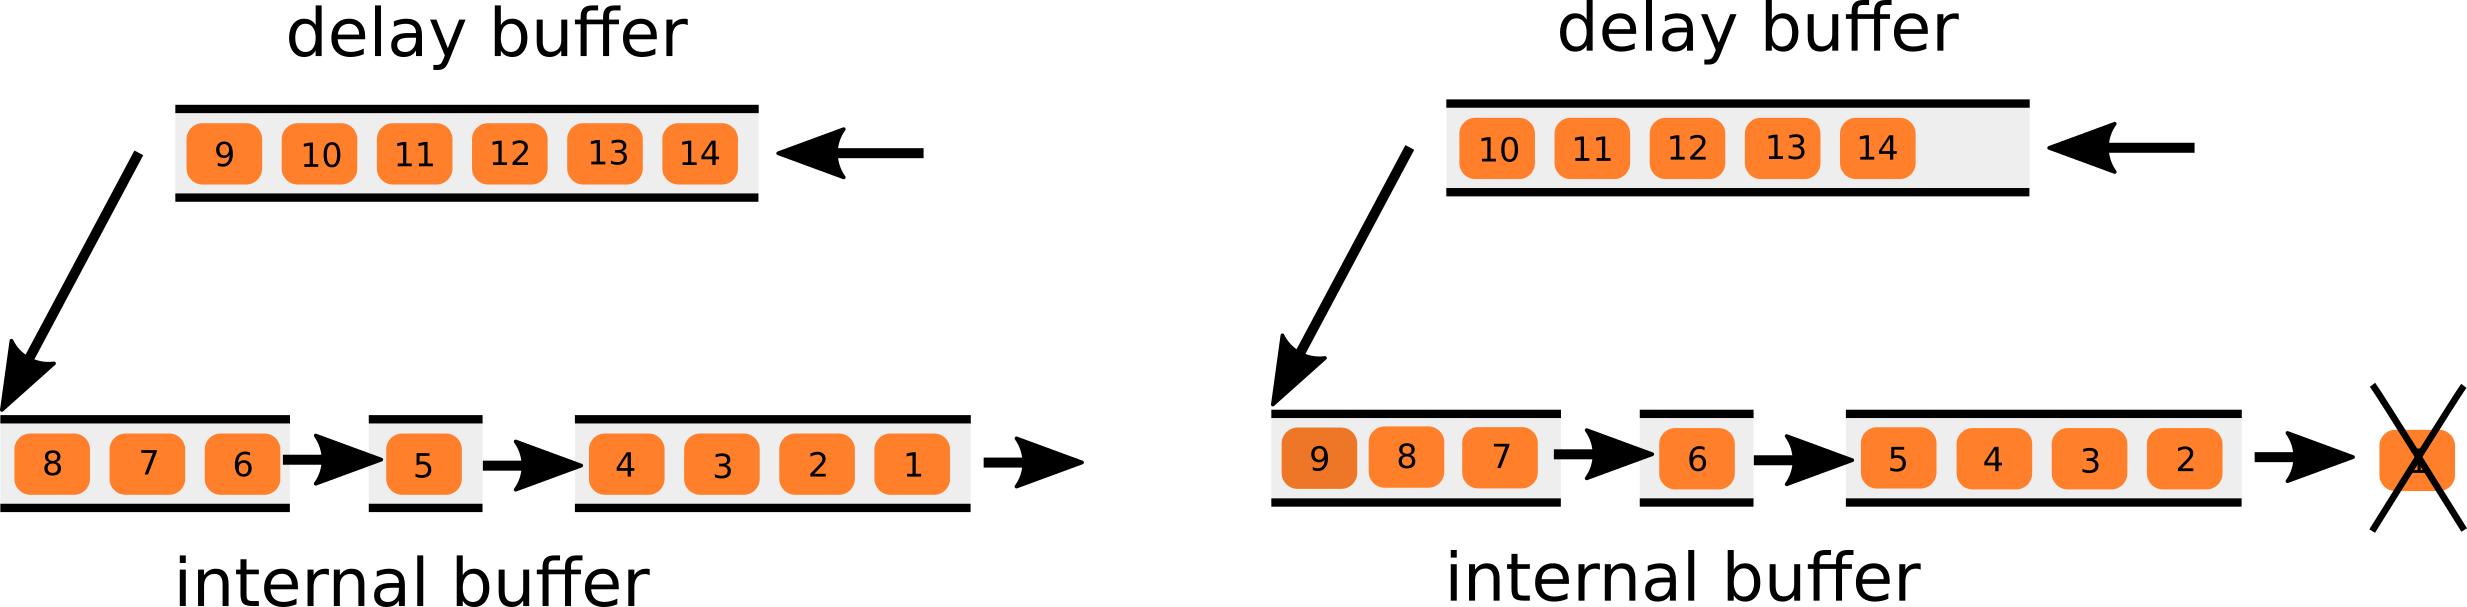
\includegraphics[height=12em]{drawings/implementation-move-forward.png}
	\caption{Move data forward.}
	\label{fig:implementation-move-forward}
\end{figure}


\paragraph{decrement\_center\_reached}
This counter (individual to each field) gets decremented every time there is a data item at the output of the delay buffer (kernel access index position [0,0,0]). The counter reaching zero indicates that the kernel reached center for this field.


\paragraph{try\_read}
This is the implementation of the kernel reading functionality of the simulator. It tries to read from all input channels and indicates if this has been done with success. It does the following procedure written in pseudo code:
\begin{algorithm}
	\caption{try\_read}
	\begin{algorithmic}
		\STATE check if all inputs are available
		\STATE case success: read all data items into the variable to value map var\_map and set the read\_success flag
		\STATE case unsucessful: reset the read\_success flag
		\STATE decrement the center counter for all fields that have data at the output of the delay queue
		\STATE check if all counter reached 0
		\STATE case true: continue
		\STATE case false: move all delay/internal buffer forward for the fields that did not reach center yet
	\end{algorithmic}
\end{algorithm}

\paragraph{try\_execute}
This is the implementation of the kernel execution functionality of the simulator. It executes the stencil computation for the current variable mapping that was set up by the try\_read() function. It does the following procedure written in pseudo code:
\begin{algorithm}
	\caption{try\_execute}
	\begin{algorithmic}
		\IF {check if center has been reached, read\_success is set and the internal program counter is between 0 and PROBLEM\_SIZE}
		\STATE get the relative access kernel string
		\STATE compute the result of the expression together with the variable map using the calculator
		\STATE add result to out\_delay\_queue
		\STATE increment the program counter
		\ELSE
		\STATE add a None (bubble) to the out\_delay\_queue
		\ENDIF
	\end{algorithmic}
\end{algorithm}


\paragraph{try\_write}
This is the implementation of the kernel write functionality of the simulator.  It does the following procedure written in pseudo code:
\begin{algorithm}
	\caption{try\_write}
	\begin{algorithmic}
		\STATE dequeue last element from the out\_delay\_queue
		\STATE add it to the input channel of all kernel outputs respectively successor nodes
	\end{algorithmic}
\end{algorithm}

\paragraph{diagnostics}
The diagnostics method summarizes the internal kernel state. It either gets called upon an exception or at the end for the final report. It provides the following information:
\begin{itemize}
	\item program counter
	\item all\_available flag
	\item center\_reached
	\item exception traceback
	\item Inputs/Outputs:
	\begin{itemize}
		\item delay buffer maximal size
		\item delay buffer current size
		\item delay buffer content
		\item internal buffer content
	\end{itemize}
	\item content of latency simulation buffer (out\_delay\_queue)
\end{itemize}


\paragraph{out\_delay\_queue}
The out\_delay\_queue's purpose is to simulate the computation latency of the computation graph. This is achieved by having a FIFO queue of length \textit{max\_latency} and by adding each result to the queue while sending out the last item from the queue each cycle instead of directly sending it out.







\section{Kernel Chain Graph (kernel\_chain\_graph.py)}
The KernelChainGraph class represents the whole pipelined data flow graph consisting of input nodes (real data input arrays, kernel nodes and output nodes (storing the result of the computation).


\paragraph{Call}
The KernelChainGraph can be called in the following way:
\begin{minted}{python}
python3 kernel_chain_graph.py -stencil_file stencils/simulator12.json -plot -simulate 
    -report -log-level 2
\end{minted}

\paragraph{Initialization}
The following procedure is called to initially setup the internal structure and analyze the input configuration:
\begin{enumerate}
	\item set up all internal data structures (dicts, lists,..)
	\item read input config files
	\item create all kernels
	\item compute kernel latencies
	\item connect kernels in the graph
	\item compute delay buffer sizes
	\item add channels to the graph edges
	\item plot all graphs (if flag set)
\end{enumerate}

\paragraph{plot\_graph}
Visualizing the stencil program instances greatly helps to get a good understanding of the problem and seeing what is going or what we could further optimize. This method accounts for that by plotting a well-arranged overview of the StencilChainGraph. 
\begin{figure}[h]
	\centering
	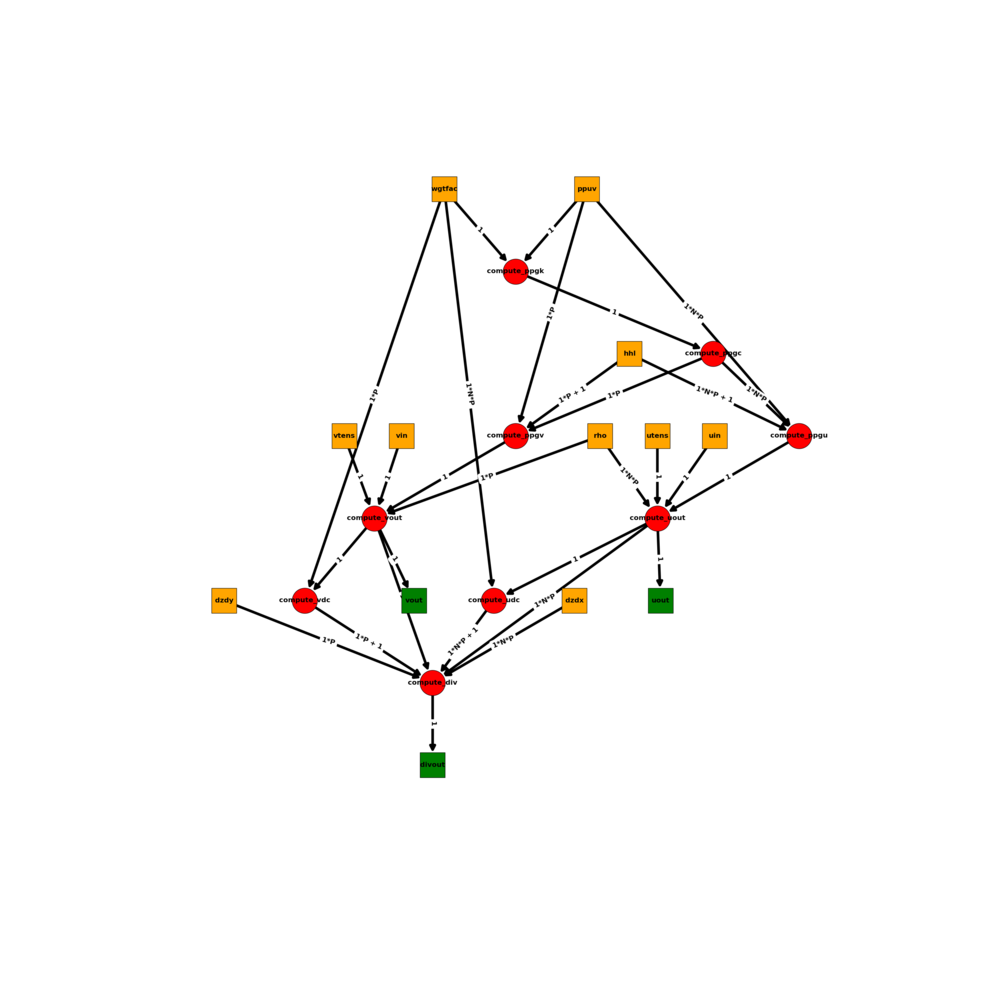
\includegraphics[height=24em]{images/fastwaves.png}
	\caption{Example stencil chain graph.}
	\label{fig:fastwaves}
\end{figure}


\paragraph{connect\_kernels}
This method connects all networkx nodes to a directed acyclic graph by matching the input names with the corresponding kernel names.


\paragraph{add\_channels}
Add\_channels packs all required information (name, delay buffer queue, internal buffer queue and data type) into a dictionary and adds it to the edge between the corresponding two nodes of the graph.
\begin{minted}{python}     
channel = {
  "name": name,
  "delay_buffer": self.kernel_nodes[dest.name].
                  delay_buffer[src.name],
  "internal_buffer": dest.internal_buffer[src.name],
  "data_type": src.data_type
}
\end{minted}


\paragraph{import\_input}
This helper method reads the input file and adds each part to the corresponding field in the class.


\paragraph{total\_elements}
Reduces the global problem size to a single scalar value.


\paragraph{create\_kernels}
Instantiates the kernels and adds them to the networkx graph.


\paragraph{compute\_kernel\_latency}
Fills a global dictionary of the individual critical kernel computation paths.


\paragraph{compute\_delay\_buffer}
Computes the delay buffer sizes in the graph by propagating all paths from the input arrays to the successors in topological order. Delay buffer entries should be of the format: kernel.input\_paths:{
	"in1": [[a,b,c, pred1], [d,e,f, pred2], ...],
	"in2": [ ... ],
	...
}
where inX are input arrays to the stencil chain and predY are the kernel predecessors/inputs. This is being achieved in the following way:
\begin{algorithm}
	\caption{compute\_delay\_buffer}
	\begin{algorithmic}
		\STATE sort the graph in topological order
		\STATE go over all nodes in the topological order
		\STATE process delay buffers (no new delay buffers can occur since its is topologically sorted)
		\STATE max delay = maximum entry for this field
		\STATE compute delay buffer for all field by subtracting it from the maximum one (the maximum one does not require a delay buffer since it is ready as the last one)
		\STATE propagate the path length as own path length + internal delay from computation and delay buffers
	\end{algorithmic}
\end{algorithm}

\begin{figure}[h]
	\centering
	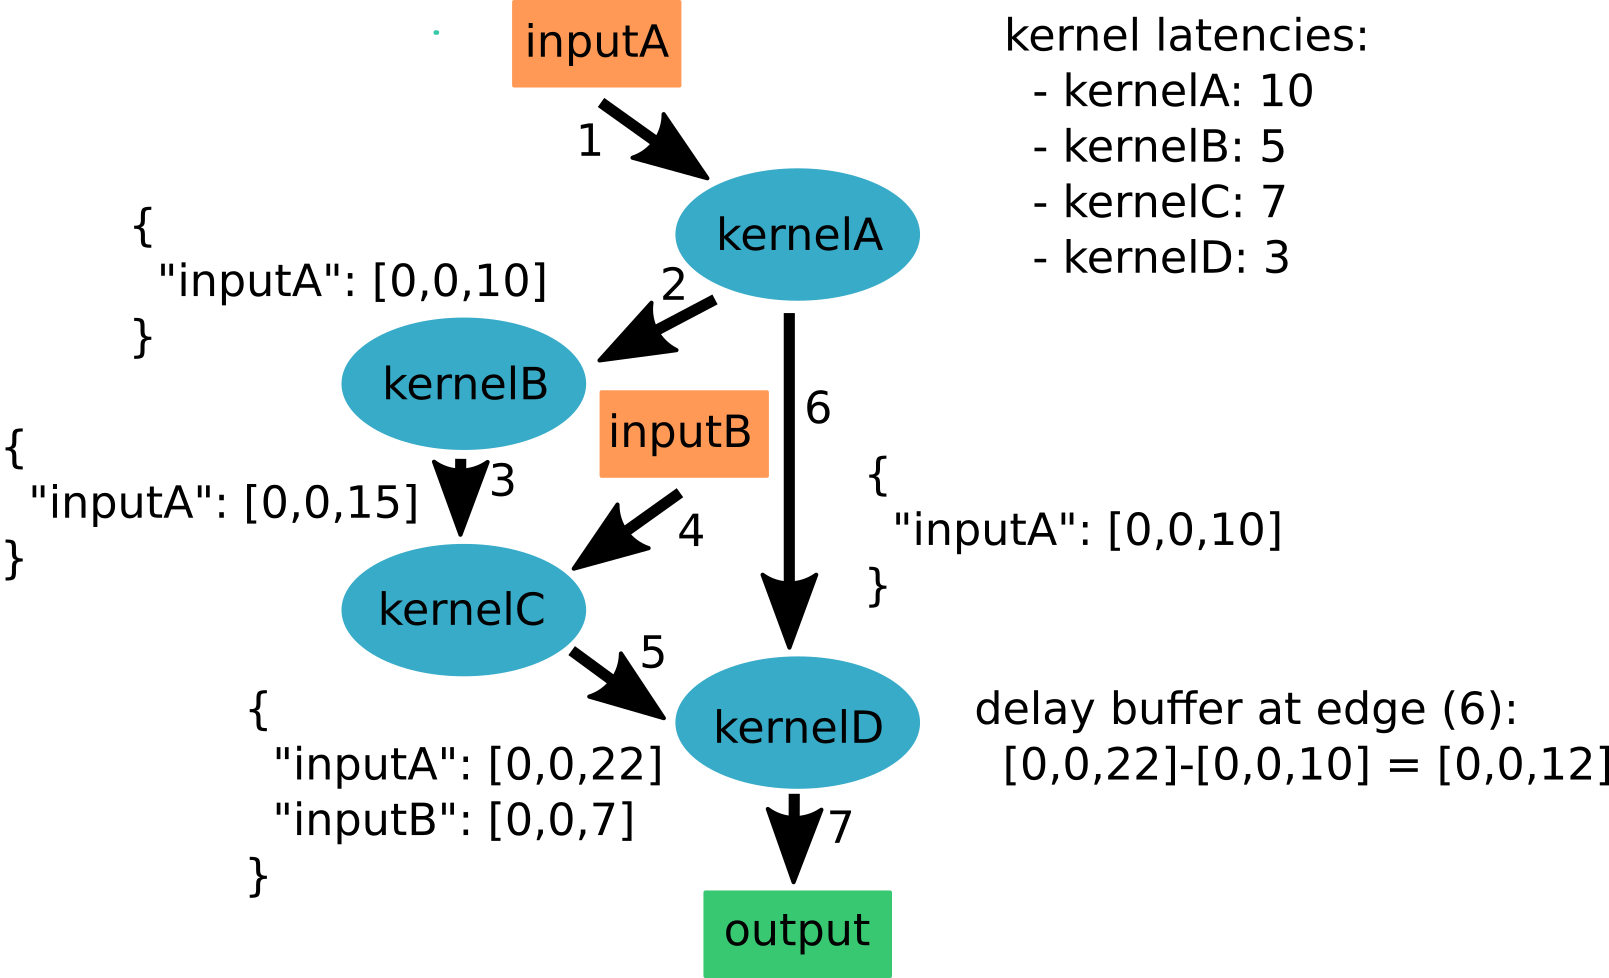
\includegraphics[height=16em]{drawings/software-delay-buffer.png}
	\caption{Example delay buffer computation using the path accesses list.}
	\label{fig:software-delay-buffer}
\end{figure}


\paragraph{compute\_critical\_path\_dim}
Computes the maximum latency critical path through the graph in dimensional format. \\
\textit{Note: Since we know the output nodes as well as the path lengths the critical path is simply
	max \{ latency(node) + max \{ path\_length(node) | node in output nodes \}\} }


\paragraph{report}
The report summarizes the stencil program information and analysis and reports the following information:
\begin{itemize}
	\item dimensions of data array (problem size)
	\item channels
	\item data field accesses
	\item internal buffer size
	\item internal buffer chunks
	\item delay buffer size
	\item path lengths (from the input to the node, per field)
	\item latency
	\item total buffer 
	\item input kernel string
	\item relative access kernel string
	\item slow and fast memory buffer size
\end{itemize}







\section{Simulator (simulator.py)}
The Simulator class handles the simulation of our high level model FPGA functionality of the stencil chain design as described in the model section (figure \ref{fig:simulator-simulation-cycle}). \\


\paragraph{simulate}
The simulate orchestrates the simulator and does the following:
\begin{algorithm}
	\caption{simulate}
	\begin{algorithmic}
		\STATE initialize: read all data into input nodes
		\STATE set global program counter PC=0
		\WHILE {not all input/kernel/output nodes done}
		\STATE step execution()
		\STATE PC = PC + 1
		\ENDWHILE
		\STATE finalize: write all output data to file
	\end{algorithmic}
\end{algorithm}

\paragraph{step\_execution}
A single step of the step\_execution represents a single cycle on an FPGA, split up into sub-steps, which are being called into the Input, Kernel and Output classes as follows:
\begin{algorithm}
	\caption{step\_execution}
	\begin{algorithmic}
		\STATE try\_read all output and kernel nodes
		\STATE try\_execute all kernel nodes
		\STATE try\_write all input and kernel nodes
	\end{algorithmic}
\end{algorithm}

\paragraph{initialize}
The initialization method does the pre-processing before the actual simulation. It takes cares care of importing the input data.


\paragraph{finalize}
The finalization method does the post-processing after successful simulation. It writes the result data to a file and outputs the performance metrics if the log-level is at least 'basic'.


\paragraph{get\_result}
The get\_result functionality allows to extract the simulation result of the stencil program to be extracted.


\paragraph{all\_done}
This method checks if all nodes have finished their execution and are idling. This is achieved by adding a local, node-internal program counter that increments whenever there has been a successful execution of an operation. For the input nodes it means: problem\_size - largest queue = program counter or in other words, as soon as the last queue is empty, the program counter reached the value of dimX*dimY*dimZ. For the kernel nodes a increment of the program counter happens after a successful execution. A program counter increment for the output node happens after a successful data read. \\
As soon as all the program counter reached the value of the problem size, we can safely terminate. Since this is a sufficient and required property, this is an efficient implementation without doing any unnecessary idle steps.


\paragraph{diagnostics}
Diagnostics in the simulator is not only an exception handler, but is actually of great importance for the whole StencilFlow tool since most of the exceptions happen because of wrong input assumptions or wrong buffer size calculations.\\
Therefore, the diagnostics exception handler does not only raise the exception, but rather starts a procedure where the current state of all nodes (input, kernel and output) is being post-processed and logged. The diagnostics function of these nodes is being called and an output log including current program counter, internal state properties (e.g. for kernel: all\_available, center\_reached, etc) and channel/buffer content is displayed. Which helps for later analysis and finding the root cause of the error.


\paragraph{report}
If the log-level is at least 'basic', a report about the internal node state is generated after the simulation successfully completed, exactly as in the diagnostic method but just without an actual exception.






\section{Optimizer (optimizer.py)}
The Optimizer class is a key piece of StencilFlow and takes care of the optimal allocation and usage of the optimization parameters: fast memory, slow memory and bandwidth. 



\paragraph{single\_comm\_volume}
This method returns the number of bytes necessary to copy a whole data array from or to the FPGA. This number actually corresponds to: dimX*dimY*dimZ * 4 bytes.


\paragraph{add\_buffers\_to\_metric}
Creates the buffer data structure for optimization. It not only stores the information about the individual buffer, its communication volume and data type, but also maintains a doubly linked list to its predecessor and successor for updating the communication volume in case of a swap\_out of a buffer.
\begin{minted}{python}
{
    "queue": entry,
    "comm_vol": 2*self.single_comm_volume(
        self.kernels[kernel].data_type.bytes),
    "type": "internal",
    "datatype_size": self.kernels[kernel].data_type.bytes,
    "prev": prev,
    "next": None
}
\end{minted}


\paragraph{max\_metric}
This method finds the buffer entry in the metric\_data list with the maximum metric value i.e. the buffer with the highest ratio: $\frac{buffer size}{communication volume}$ that is still located in fast memory.


\paragraph{ratio}
Computes the ratio between fast memory and the communication volume of the current optimization state. This is useful for the \textit{optimize\_to\_ratio} optimization strategy.


\paragraph{update\_comm\_vol}
This method is being called for both neighbors if we moved a fast memory buffer to the slow memory. It updates the communication volume according to the formula derived in the model section according to the following rule:
\begin{lstlisting}[showstringspaces=false, frame=single, language=Python]
How to determine the necessary communication volume?
(predecessor, successor):
case (fast, fast): 2*C
case (fast, slow): C
case (slow, fast): C
case (slow, slow): 0
where C:= communication volume to stream single data
    array in or out of fast memory (=SIZE(data array))
\end{lstlisting}
\textit{Note: pred of delay buffer is always fast memory since the stream from the predecessor kernel is being compute on the FPGA die next to the fast memory.}


\paragraph{minimize\_comm\_vol}
This optimization strategy optimizes the problem to minimize the communication volume between fast and slow memory. In other words, it uses as little bandwidth as possible by a given amount of fast and slow memory. This implies that this strategy makes maximal use of the fast memory. The pseudo code for this function is:
\begin{algorithm}
	\caption{minimize\_comm\_vol(fast\_memory\_bound, slow\_memory\_bound)}
	\begin{algorithmic}
		\STATE mark all buffers to be allocated in fast memory
		\WHILE {metric\_data list is not empty and fast\_memory\_use > fast\_memory\_bound}
		\STATE swap max metric buffer to slow memory
		\STATE update neighbors
		\STATE remove buffer from metric\_data
		\STATE update fast memory, slow memory and bandwidth use
		\IF {check if slow\_memory\_use > slow\_memory\_bound}
		\STATE Exception
		\ENDIF
		\ENDWHILE
	\end{algorithmic}
\end{algorithm}

\textit{Note: The above exception occurs if the total buffer memory consumption is higher than sum of the slow memory and fast memory bound, which means that there cannot be found any solution for this optimization problem.}


\paragraph{minimize\_fast\_mem}
This optimization strategy minimizes the usage of fast memory by a given amount of communication volume from/to slow memory. This implies that strategy makes maximal use of the available memory bandwidth and slow memory. The pseudo code for this function is:
\begin{algorithm}
	\caption{minimize\_fast\_mem(communication\_volume\_bound, slow\_memory\_bound)}
	\begin{algorithmic}
		\STATE mark all buffers to be allocated in fast memory
		\WHILE {metric\_data list is not empty and comm\_volume\_use > comm\_volume\_bound and slow\_memory\_use < slow\_memory\_bound}
		\STATE swap max metric buffer to slow memory
		\STATE update neighbors
		\STATE remove buffer from metric\_data
		\STATE update fast memory, slow memory and bandwidth use
		\ENDWHILE
	\end{algorithmic}
\end{algorithm}

\paragraph{optimize\_to\_ratio}
This optimization strategy optimizes for the given ratio value between the fast memory usage and the amount of available communication volume. The pseudo code for this function is given by:
\begin{algorithm}
	\caption{optimize\_ratio(ratio)}
	\begin{algorithmic}
		\STATE mark all buffers to be allocated in fast memory
		\WHILE {metric\_data list is not empty and current\_ratio > ratio}
		\STATE swap max metric buffer to slow memory
		\STATE update neighbors
		\STATE remove buffer from metric\_data
		\STATE recompute current\_ratio
		\STATE update fast memory, slow memory and bandwidth use
		\ENDWHILE
	\end{algorithmic}
\end{algorithm}

\paragraph{report}
The optimizer report gives an overview of the important metric values such as:
\begin{itemize}
	\item swap status: which buffers are swapped out to slow memory and which are allocated in fast memory
	\item fast memory usage (for the strategy we optimized for)
	\item slow memory usage (for the strategy we optimized for)
	\item communication volume usage (for the strategy we optimized for)
\end{itemize}







\section{SDFG Generator (sdfg\_generator.py)}
The Stateful DataFlow multiGraph (SDFG) Generator is the interface between the high-level representation in StencilFlow and the low-level and hardware design generator in DaCe \cite{label57}. This part has been implemented by my mentor Johannes de Fine Licht.







\section{Run Program (run\_program.py)}
Run\_program is a wrapper program that instantiates all required components and classes in order to run the input stencil program with the given input data arrays in software or hardware as specified by the arguments. Furthermore, we can simulate the design using StencilFlow and check if the output matches.
\begin{enumerate}
	\item read program input file
	\item create the kernel chain graph (including analysis of buffer sizes, latencies, etc)
	\item execute the optimizer
	\item execute the simuator and store the result
	\item generate HLS OpenCl code from the high-level representation (using SDFG)
	\item compile the code
	\item read input data arrays
	\item run the design in hardware (or in the Intel SDK Simulation Mode)
	\item compare the result to the output from the simulator and check if they match
\end{enumerate}

\textit{Note: In order to run the design on the actual hardware, we have to do the synthesis from the OpenCL code to the actual hardware bitstream. This is being done separately since we have to do this only once and since it takes many hours and should therefore not block the very limited number of nodes with hardware FPGAs installed.}


\section{Helper (helper.py)}
The helper name space does not contain any specific classes, but rather very helpful and highly reused utility functions. \\
The most important ones are: \\
\textit{str\_to\_dtype} In order to have a simpler interaction with DaCe, we use their data type class throughout the project. This method provides the functionality to convert generic strings of data type names (e.g. "float64") to DaCe data types.\\

\textit{parse\_json} Reads the input file from disk and parses the json as a python dictionary including some pre-processing (data type conversion) and sanity checks (e.g. file exist).

\textit{max\_dict\_entry\_key} Returns the key of the largest value entry of the input dictionary. 

\textit{list\_add\_cwise} Adds all items of two lists component-wise.

\textit{list\_subtract\_cwise} Subtracts all items of two list component-wise. 

\textit{dim\_to\_abs\_val} Computes the scalar number from the dimensional input using the global array dimensions (problem size). i.e. dim [X, Y, Z], size [a, b, c] $->$ 1*c + X*(b + Y*a) = [a, b, c] * transpose([Z*Y, Z, 1]). 

\textit{load\_array} Loads arrays of various input formats. 

\textit{save\_array} Stores numpy arrays to file. 

\textit{load\_input\_arrays / save\_output\_arrays} Basic functionality for loading actual data from file for transfer to the FPGA and store it back to the filing system.


\textit{arrays\_are\_equal} Checks if two arrays are equal (up to  some tolerance). This is used e.g. for verification of simulator output and the actual hardware output. 

\textit{unique} Removes duplicates from the given iterable.






\section{Log-Level (log\_level.py)}
As the tool chain was growing and the combination of different functionalities accumulated it became apparent that we need a clever scheme for managing the verbosity of the output console log messages. We decided to implement this using log levels as follows:
\begin{itemize}
	\item level 0: no logging
	\item level 1: basic logging (output what the program is doing)
	\item level 2: moderate logging (output what the program is doing and basic information about the actual content it is processing)
	\item level 3: full logging (output what the program is doing and full information disclosure, including e.g. program counter and buffer content of every stencil program during simulation)
\end{itemize}
Each lower log level is a subset of the higher log level. It is usually helpful to get a good trade-off between these levels depending on the purpose, since e.g. simulation performance suffers a lot under log-level 3 performance-wise.






\section{Testing (testing.py)}
As the project progressed, software complexity increased significantly which makes it prone to bugs, especially while refactoring. Furthermore, the integration of DaCe and the parallel work of my mentor Johannes de Fine Licht and me on related software made it necessary to ensure proper code functionality in the master branch. Therefore and because we want to achieve good software practices, we decided to do extensive testing for the low level functionality (e.g. bounded queue) and basic function testing for the remaining parts. This way, we can ensure that changes did not break anything before actually checking them in potentially preventing someone from being able to work.






\section{Dynamical Core Estimate (dycore\_estimate.py)}
The dynamical core estimate program is not part of StencilFlow used for internal functionality, but has rather been used to do a half-automatic walk-through of computing the required numbers for the estimate. It instantiates the KernelChainGraph for the three stencil programs (fastwaves, advection and diffusion) we used in order to compute the mean as well as for getting the delay buffer estimate for the full dynamical core. 
